\chapter{Architectural Design}
This section aims to present and analyze the architecture of the S2B in a top-down manner. 
We discuss about the architectural design choices and the reasons behind them. 

\section{Overview: High-level components and their interactions}
The figure shown below represents a high-level description of the components which make up the system.
\begin{figure}[H]
    \centering
    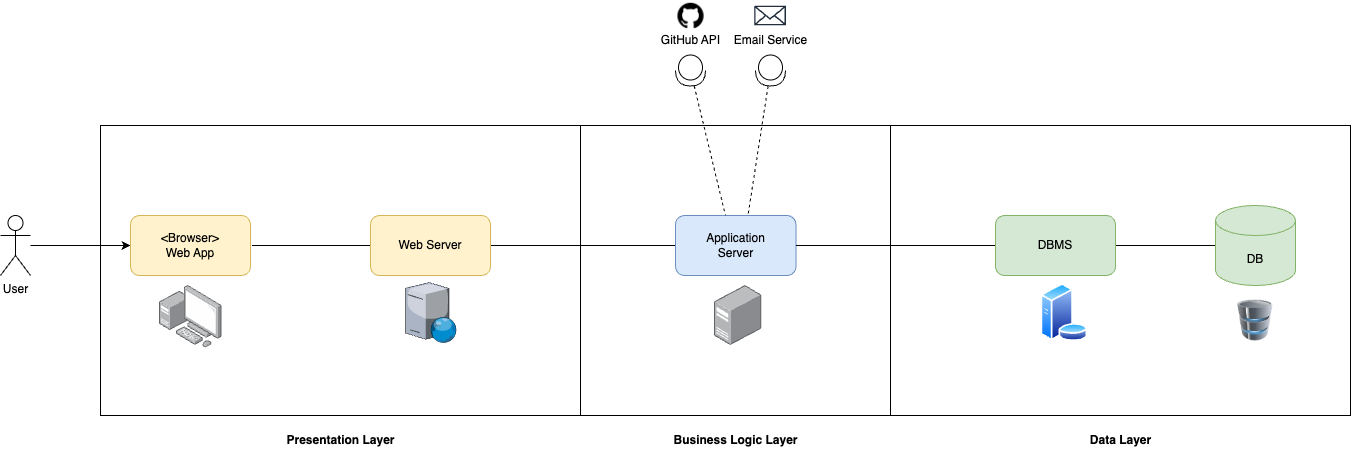
\includegraphics[width=\textwidth]{images/component_view/high_level.png}
    \caption{Overview CKB architecture}
    \label{fig:CKB Architecture}
\end{figure}
A web interface will be used to access the platform. 
The overall architecture of the system is based on a three-tier architecture, 
with the application servers interacting with a database management system and
using APIs to retrieve and store data. \\
The three logical layers corrspond to three different physical layers and each layer can communicate only with the adjacent ones.
The interactions between clients and server are stateless according to the REST architectural style. \\
The web server is responsible for the communication with the clients and for the management of the requests. \\
The application server holds the business logic of the application and it can communicate with the database server to retrieve and store data, also with the GitHub platform and the Email Service. 

\section{Component view}

\subsection{High level view}
\begin{figure}[H]
    \centering
    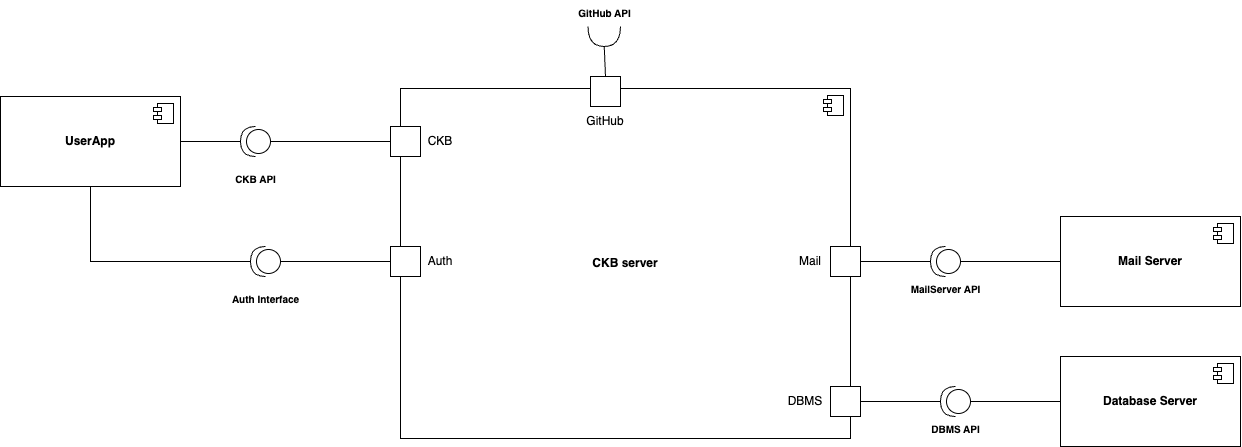
\includegraphics[width=\textwidth]{images/component_view/Component_view.png}
    \caption{High level component view}
\end{figure}
The figure above shows the system components and interfaces at a high level.
\begin{itemize}
    \item \textbf{CKB Server: } it represents the core of the CKB system and it contains all the business logic.
    \item \textbf{UserApp: } it represents the web application used by the users to access the CKB platform. Users register and log into the system through the 
    \textbf{Auth interface} and access the functionalities offered by the system through the \textbf{CKB API}.
    \item \textbf{Database Server: } it represents the DBMS used to store the data of the system. The system can access the data through the \textbf{DBMS API}.
    \item \textbf{Mail Server: } it represents the mail server used to send notifications to the users. The system can access the mail server through the \textbf{MailServer API}.
\end{itemize}

\subsection{CKB Server detailed view}
\begin{figure}[H]
    \centering
    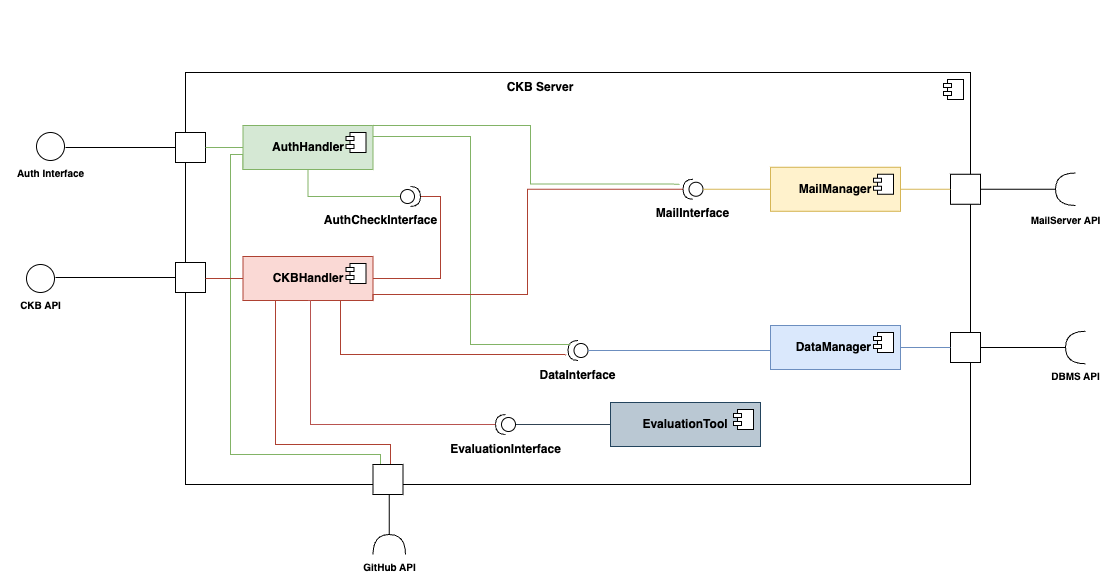
\includegraphics[width=\textwidth]{images/component_view/CKB_component.png}
    \caption{CKB server component view}
\end{figure}
The figure above shows the internal componenents of the CKB server.
\begin{itemize}
    \item \textbf{AuthHandler: } it handles the login and registration of the users. It offers the \textbf{AuthCheckInterface} to allow other components to check 
    if a user is authorized. It communicates with the \textbf{MailInterface} to manage confirmation emails and with the \textbf{DataInterface} to check the credentials
    correctness.
    \item \textbf{CKBHandler: } it handles all the functionalities offered by the system. It communicates with the \textbf{DataInterface} to retrieve and store data, with 
    the \textbf{AuthCheckInterface} to check if a user is authorized to perform a certain operation and with the \textbf{MailInterface} to send notifications to the users.
    It also communicates with the \textbf{GitHubInterface} to retrieve data (nickname and pushed code) from the GitHub platform.
    \item \textbf{MailManager: } it handles the access to the mail server, it provides the \textbf{MailInterface} that allows components to send emails.
    \item \textbf{DataManager: } it handles the access to the persistent data saved on the DB, almost every component communicates with it through the \textbf{DataInterface}.
\end{itemize}


\subsection{Auth component view}
\begin{figure}[H]
    \centering
    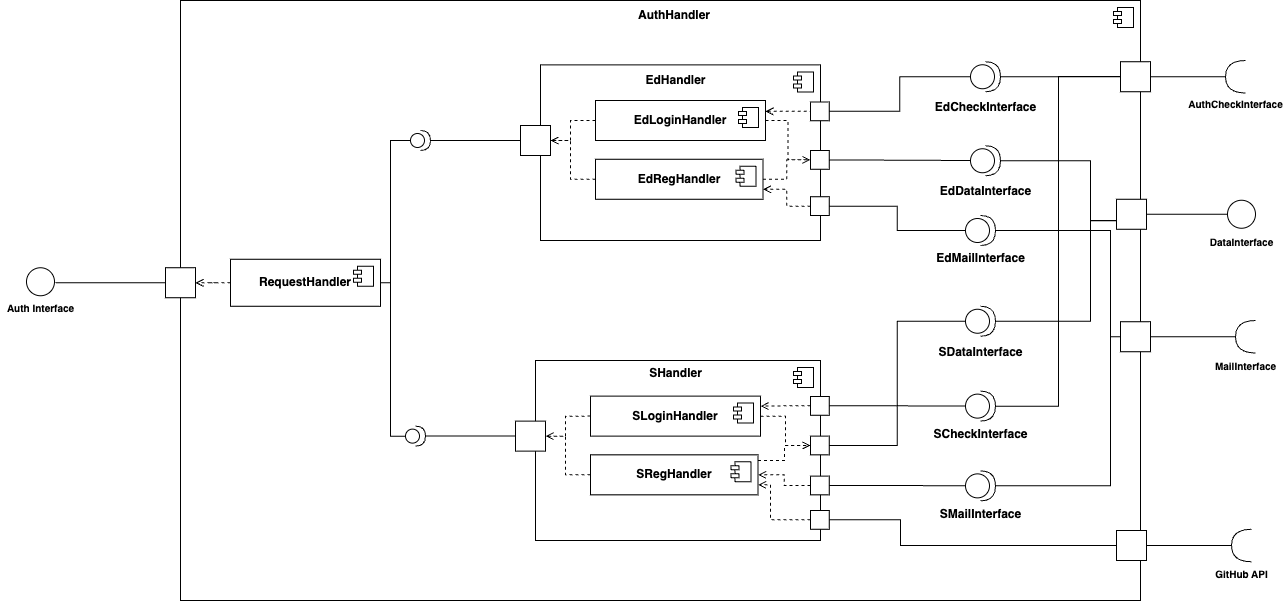
\includegraphics[width=\textwidth]{images/component_view/Auth.png}
    \caption{Auth component view}
\end{figure}
The figure above shows the internal componenents of the AuthHandler.
\begin{itemize}
    \item \textbf{RequestHandler: } it handles the requests acting as a router dispatching requests to the right handler.
    \item \textbf{EdHandler: } it is composed by the \textbf{EdLoginHandler} and the \textbf{EdRegHandler}. The former handles the login of educators, 
    the latter handles their registration.
    \item \textbf{SHandler: } it is composed by the \textbf{SLoginHandler} and the \textbf{SRegHandler}. The former handles the login of students,
    the latter handles their registration.
\end{itemize}
LoginHandlers communicate with the \textbf{AuthCheckInterface} to check the authorization of a user.\\
RegistrationHandlers communicate with the \textbf{MailInterface} to send confirmation emails and with the \textbf{DataInterface} to store the data of the new user.\\
SRegistrationHandler also communicate with \textbf{GitHubAPI} to link the CKB account with the GitHub one.

\section{Deployment view}
The figure below shows the architecture of the system. All the users access to the WebApp through the browser, which communicate with
the Web Server. Both Web Server and Application Server are hosted on a Cloud Provider. This choice offers many
advantages, such as:

\begin{itemize}
    \item  \textbf{Scalability and flexibility: }the ability of adding and removing resources efficiently throw 
    the use of load balancing services which allows the application server to manage traffic and workload. 
    \item   \textbf{Security: }the ability to protect the application server using firewall and DMZ, againist cyberattacks and possible threats.
    \item   \textbf{Cost efficiency:} the ability to pay only for the resources used which can help to lower the overall cost. 
\end{itemize}

\begin{figure}[H]
    \centering
    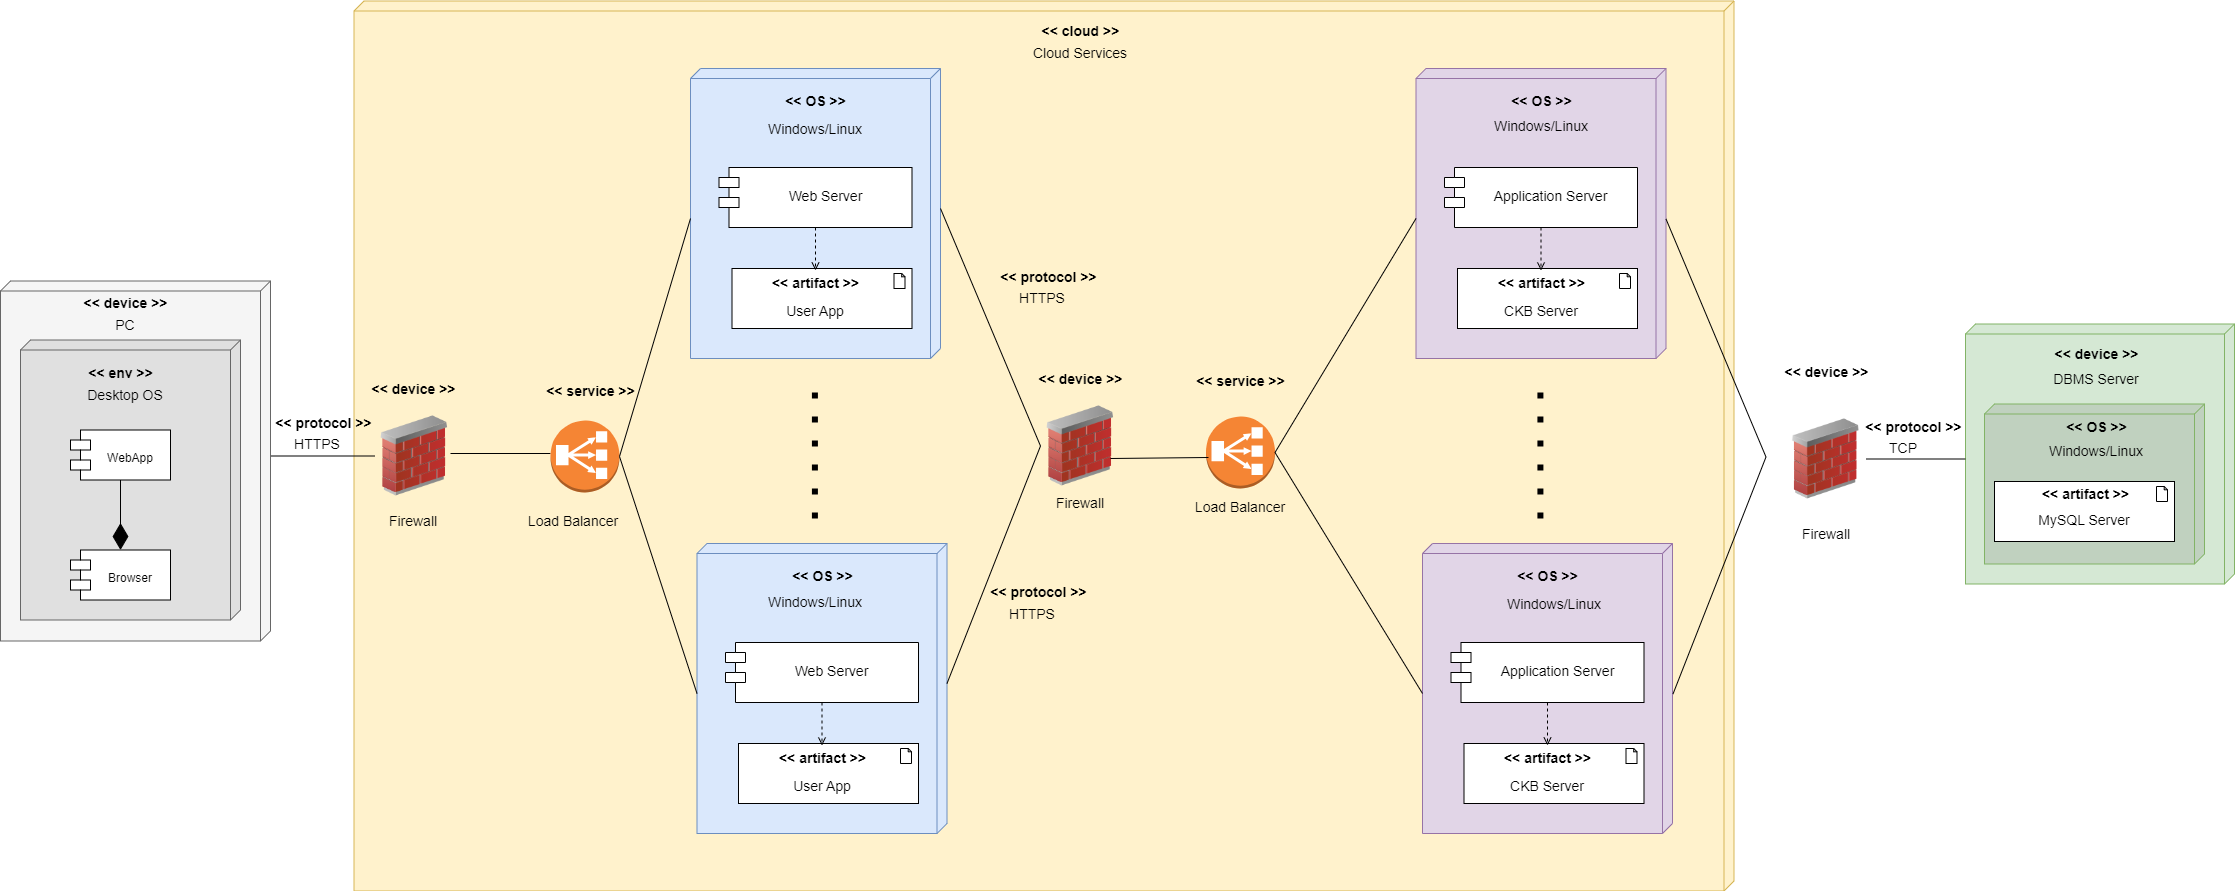
\includegraphics[width=1\textwidth]{images/Deployment_diagram.png}
    \caption{Deployment diagram}
\end{figure}

The deployment diagram offers a more detailed view over the hardware and software components of the system. 
\begin{itemize}
    \item  \textbf{PC: }is any device having a browser capable of running the JavaScript code.
    \item   the Cloud Services will host all the business and data logic for the system. It is characterized by 
    \begin{itemize}
        \item  \textbf{Firewall:} devices are used to protect and filter incoming connections to the logic and data layers of the system. It protects the system from unauthorized access and malicious attacks.
        \item  \textbf{Load Balancer:} services are used to distribute the workload across multiple servers. It helps to improve the performance and reliability of the system. It also helps to ensure that application can handle a large volume of requests, without any downtime.
        \item  \textbf{Multiple copies of Web Server and Application Server:} are used to ensure that the system is always available. The different instances can be created and destroyed dynamically, based on the workload. It also helps to achieve fault tolerance by allowing traffic to be redirect to a different instance, if one instance becomes unavailable.
    \end{itemize}
    \item   \textbf{Database:} is used to store all the data of the system. It uses MySQL as DBMS to retrieve and store data.
    \item   \textbf{Mail Provider: }is used to send notifications to the users. It uses Gmail as mail provider.
\end{itemize}
\section{Runtime view}
\section{Component interfaces}
\section{Selected architetural styles and patterns}
\section{Other design decisions}